\documentclass[12pt,a4paper]{article}
\usepackage[utf8]{vietnam}
\usepackage{amsmath,amsfonts,amssymb}
\usepackage{graphicx}
\usepackage{enumerate}
\usepackage{fontawesome}

\usepackage{tikz}
\usetikzlibrary{math,through,calc,intersections,angles,quotes,shapes,shapes.geometric,arrows,patterns,snakes,matrix,chains,arrows.meta,decorations.shapes,decorations.fractals,decorations.markings,shadows}
\usepackage{longtable,multirow,makecell}
\usepackage{arydshln}
\usepackage{diagbox}

\usepackage[loigiai]{ex_test}

\usepackage[left=1.5cm, right=1.5cm, top=1.5cm, bottom=1.5cm]{geometry}

\renewcommand{\labelitemi}{\faFacebookOfficial}
\renewcommand{\labelitemii}{\faAmazon}

\renewcommand{\labelenumi}{\Roman{enumi})}
\renewcommand{\labelitemii}{\faAmazon}
\def\canhgiua{\centering\arraybackslash}

\setlength{\parindent}{0pt}


\begin{document}

\begin{minipage}[t]{7cm}
	\begin{center}
		\textbf{BỘ GIÁO DỤC VÀ ĐÀO TẠO \\[3pt]
			ĐỀ CHÍNH THỨC}
	\end{center}
\end{minipage}
\hspace{3cm}
\begin{minipage}[t]{7cm}
	\begin{center}
		\textbf{ĐỀ KIỂM TRA\\[3pt]
			Môn: VẬT LÍ}
	\end{center}
\end{minipage}\\[6pt]

\textbf{Phần I. Câu hỏi trắc nghiệm nhiều phương án lựa chọn.}

\begin{ex}
	Một lượng khí được giữ ở một nhiệt độ xác định, khi áp suất là $10^5$ Pa thì có thể tích 6 lít, khi áp suất là $1,5.10^5$ Pa thì có thể tích là
	\choice
	{12 lít}
	{8 lít}
	{4 lít}
	{9 lít}
\end{ex}

\begin{ex}
	Một xilanh chứa $150 \text{ cm}^3$ khí ở áp suất $1,2.10^5$ Pa. Piston nén đẳng nhiệt khí trong xilanh đến thể tích $100 \text{ cm}^3$ thì áp suất của khí là
	\choice
	{$0,8.10^5$ Pa}
	{$1,8.10^5$ Pa}
	{$1,5.10^5$ Pa}
	{$0,5.10^5$ Pa}
\end{ex}

\begin{ex}
	Một lượng khí lí tưởng được nén đẳng nhiệt từ 8 lít xuống 6 lít thì áp suất thay đổi một lượng là $1,2.10^5$ Pa. Áp suất ban đầu của khí là
	\choice
	{$1,6.10^4$ Pa}
	{$4,8.10^4$ Pa}
	{$0,9.10^5$ Pa}
	{$3,6.10^5$ Pa}
\end{ex}

\begin{ex}
	Một xe tải khi không chở hàng thì thể tích khí trong lốp là $V_0$ và $P_0$. Sau khi xếp hàng lên thì áp suất trong lốp tăng thêm một lượng $\Delta P$. Coi khí trong lốp là lí tưởng, khối lượng và nhiệt độ của nó không thay đổi. Thể tích của khí trong lốp sau khi xếp hàng lên xe là
	\choice
	{tăng thêm $\dfrac{\Delta P.V_0}{P_0 + \Delta P}$}
	{giảm đi $\dfrac{\Delta P.V_0}{P_0 + \Delta P}$}
	{tăng thêm $\dfrac{\Delta P.V_0}{P_0 - \Delta P}$}
	{giảm đi $\dfrac{\Delta P.V_0}{P_0 - \Delta P}$}
\end{ex}

\begin{ex}
	Một lượng khí lí tưởng ban đầu có áp suất $p_1$. Giữ nhiệt độ của khí không đổi nhưng tăng áp suất thêm một lượng $0,5p_1$ thì thể tích của khí thay đổi một lượng 2 lít. Thể tích ban đầu của khí là
	\choice
	{1 lít}
	{4 lít}
	{6 lít}
	{3 lít}
\end{ex}

\begin{ex}
	Một lượng khí lí tưởng xác định, ban đầu ở áp suất 3 atm. Bây giờ giữ nhiệt độ của khí không đổi đồng thời tăng áp suất khí thêm 2 atm thì thể tích khí thay đổi một lượng 4 lít. Thể tích ban đầu của khí là
	\choice
	{2 lít}
	{4,4 lít}
	{10 lít}
	{6 lít}
\end{ex}

\begin{ex}
	Trong bể nước có nhiệt độ không đổi, một bong bóng khí nổi dần lên từ đáy bể. Trong quá trình nổi lên thể tích và áp suất của bong bóng khí thay đổi như thế nào?
	\choice
	{Thể tích tăng và áp suất giảm}
	{Thể tích và áp suất đều không đổi}
	{Thể tích và áp suất đều tăng}
	{Thể tích và áp suất đều giảm}
\end{ex}

\begin{ex}
	Một bong bóng khí có thể tích $V$ nằm ở đáy ao, nổi dần lên trên mặt nước. Biết ao nước sâu 3 m, nước có nhiệt độ không đổi, áp suất khí quyển là $10^5$ Pa, khối lượng riêng của nước là $10^3 \text{ kg/m}^3$. Thể tích của bong bóng khí này khi ở mặt nước là
	\choice
	{$1,3V$}
	{$1,5V$}
	{$0,7V$}
	{$0,5V$}
\end{ex}

\begin{ex}
	Một bong bóng khí nổi dần từ đáy hồ lên mặt nước thì thể tích tăng lên gấp đôi. Biết nhiệt độ nước hồ không đổi, áp suất khí quyển là $10^5$ Pa, khối lượng riêng của nước là $1000 \text{ kg/m}^3$ và $g = 10 \text{ m/s}^2$. Độ sâu của nước là
	\choice
	{10 m}
	{20 m}
	{5 m}
	{4 m}
\end{ex}

\begin{ex}
	Một bình đang chứa khí ở áp suất 1,0 atm và thể tích 6,0 lít, được bơm thêm một lượng khí có thể tích 9,0 lít và áp suất 1,0 atm. Giả sử rằng quá trình bơm khí có nhiệt độ không đổi. Áp suất khí trong bình chứa không khí sau đó là
	\choice
	{1,0 atm}
	{1,5 atm}
	{2,0 atm}
	{2,5 atm}
\end{ex}

\begin{ex}
	Dùng bình chứa khí lí tưởng có áp suất 24 atm và thể tích 20 lít để bơm từ từ vào 15 bình chân không có thể tích 20 lít, quá trình bơm bình cuối cùng dừng lại tự nhiên. Coi nhiệt độ không đổi trong quá trình bơm và áp suất trong các bình được bơm bằng nhau. Áp suất bên trong các bình được bơm là
	\choice
	{1,5 atm}
	{1,6 atm}
	{2,4 atm}
	{1,2 atm}
\end{ex}

\begin{ex}
	Một bình khí oxy có thể tích 20 lít và áp suất là 30 atm được mở van để cho oxy phân phối vào các lọ chân không có thể tích 5 lít. Áp suất trong các lọ sau khi phân phối là 2 atm. Biết quá trình phân phối nhiệt độ không đổi và không có rò rỉ khí. Số lọ có thể phân phối là
	\choice
	{4}
	{50}
	{56}
	{60}
\end{ex}

\begin{ex}
	Một bình oxy cao áp có áp suất $1,3.10^7$ Pa và thể tích 30 lít. Mỗi ngày cần lấy ra từ bình một lượng khí có thể tích 400 lít ở áp suất $1,0.10^5$ Pa. Coi nhiệt độ khí không thay đổi. Để đảm bảo áp suất của oxy trong bình không nhỏ hơn $1,0.10^6$ Pa thì lượng oxy trong bình có thể sử dụng
	\choice
	{3 ngày}
	{6 ngày}
	{9 ngày}
	{12 ngày}
\end{ex}

\begin{ex}
	Để thuận tiện rút thuốc từ lọ thuốc kín, y tá thường sử dụng ống tiêm để bơm một lượng nhỏ khí vào lọ thuốc. Như hình vẽ, một chai thuốc có thể tích 0,9 ml và chứa 0,5 ml thuốc, áp suất của khí trong lọ là $10^5$ Pa. Một lượng khí trong ống tiêm có tiết diện $0,3 \text{ cm}^2$, dài 0,4 cm và áp suất $10^5$ Pa được y tá bơm vào lọ thuốc. Biết nhiệt độ bên trong và bên ngoài lọ thuốc bằng nhau và không thay đổi. Áp suất của lượng khí mới trong lọ thuốc là
	\begin{center}
		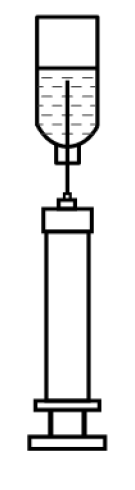
\includegraphics[scale=0.3]{img/1.png}
	\end{center}
	\choice
	{$7,7.10^4$ Pa}
	{$1,3.10^5$ Pa}
	{$7,5.10^4$ Pa}
	{$1,5.10^5$ Pa}
\end{ex}

\begin{ex}
	Áp suất lốp là một thông số quan trọng phải lưu tâm để lái xe an toàn. Thể tích lốp của một ô tô là 25 lít và phạm vi áp suất lốp an toàn là từ 2,4 atm đến 3,0 atm. Sau khi ô tô chạy một thời gian, người lái xe thấy áp suất lốp giảm xuống 2,0 atm nên sử dụng máy bơm không khí trên xe có tốc độ bơm là 0,5 lít khí ở áp suất 1,0 atm mỗi giây. Bỏ qua sự thay đổi thể tích lốp và nhiệt độ khí. Khoảng thời gian bơm không khí để đưa áp suất lốp về mức an toàn là
	\choice
	{từ 120 s đến 150 s}
	{từ 60 s đến 75 s}
	{từ 40 s đến 100 s}
	{từ 20 s đến 50 s}
\end{ex}

\begin{ex}
	Một xilanh tiết diện $20 \text{ cm}^2$, được đặt nằm ngang, trong ống là một lượng khí nhất định được bao bởi piston có thể trượt không ma sát trong ống. Áp suất khí quyển là $10^5$ Pa. Ban đầu, cột khí trong ống dài là 18 cm. Dùng lực đẩy ngang từ từ đẩy piston di chuyển sang trái 3 cm. Coi nhiệt độ khí không đổi. Lúc này, lực đẩy lên piston có độ lớn là
		\begin{center}
		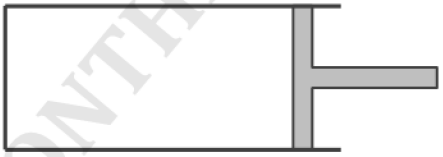
\includegraphics[scale=0.3]{img/2.png}
	\end{center}
	\choice
	{50 N}
	{20 N}
	{40 N}
	{30 N}
\end{ex}

\begin{ex}
	Một piston có khối lượng không đáng kể được giữ trong một xilanh thẳng đứng tiết diện $S = 5 \text{ cm}^2$, dưới piston là một lượng khí lí tưởng có thể tích $6.10^{-5} \text{ m}^3$ (hình H1). Tác dụng lực F lên piston để nén khí từ từ (hình H2), nhiệt độ của khí không đổi. Biết áp suất khí quyển là $10^5$ Pa và $g = 10 \text{ m/s}^2$. Khi $F = 25$ N thì thể tích khí trong xilanh là
		\begin{center}
		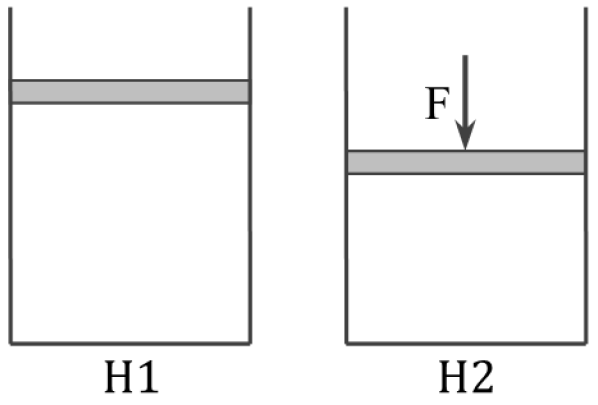
\includegraphics[scale=0.3]{img/3.png}
	\end{center}
	\choice
	{$3.10^{-5} \text{ m}^3$}
	{$5.10^{-5} \text{ m}^3$}
	{$8.10^{-5} \text{ m}^3$}
	{$4.10^{-5} \text{ m}^3$}
\end{ex}

\begin{ex}
	Một lượng khí được chứa trong một xilanh có khối lượng $M$ và một piston có khối lượng $m$ và diện tích $S$. Không có ma sát và sự rò rỉ khí giữa piston và xilanh. Khi xilanh đặt nằm ngang (hình H1) thì chiều dài của cột không khí là $L_0$. Nếu xilanh được treo thẳng đứng (hình H2) thì chiều dài của cột không khí bao nhiêu? Biết áp suất khí quyển là $p_0$ và nhiệt độ của khí không đổi.
		\begin{center}
		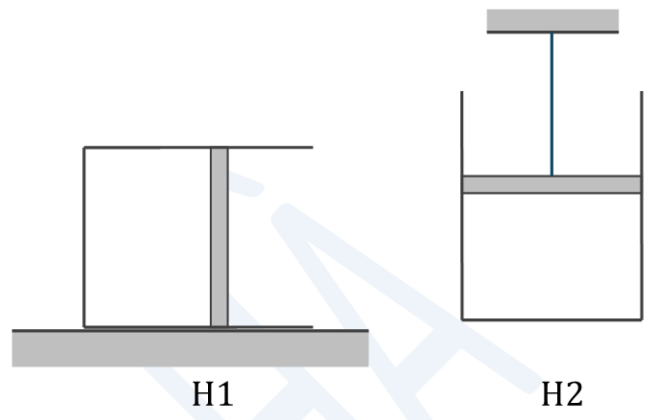
\includegraphics[scale=0.3]{img/4.png}
	\end{center}
	\choice
	{$\dfrac{p_0S-Mg}{p_0S}L_0$}
	{$\dfrac{p_0S}{p_0S+Mg}L_0$}
	{$\dfrac{p_0S}{p_0S-Mg}L_0$}
	{$\dfrac{p_0S+Mg}{p_0S}L_0$}
\end{ex}

\begin{ex}
	Một xilanh có khối lượng $m$ và tiết diện $S$ được đặt trên mặt bàn nằm ngang, piston và tay cầm của nó có khối lượng $m_0$, dưới piston là một lượng khí lí tưởng. Ban đầu piston đứng yên ở độ cao $h$ tính từ đáy xilanh. Biết áp suất khí quyển là $p_0$. Nâng piston từ từ lên trên, bỏ qua ma sát và sự thay đổi nhiệt độ của khí. Khi piston được nâng lên một đoạn so với ban đầu là bao nhiêu thì xilanh rời khỏi mặt bàn?
		\begin{center}
		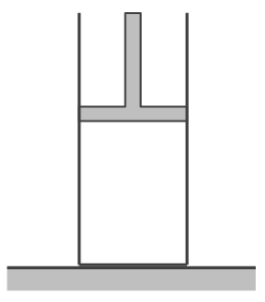
\includegraphics[scale=0.3]{img/5.png}
	\end{center}
	\choice
	{$\dfrac{m_0g+mg}{p_0S-mg}h$}
	{$\dfrac{m_0g+mg}{p_0S-m_0g}h$}
	{$\dfrac{p_0S-m_0g}{m_0g+mg}h$}
	{$\dfrac{p_0S-mg}{m_0g+mg}h$}
\end{ex}

\begin{ex}
	Một xilanh đặt thẳng đứng, đầu hở phía trên, chứa cột khí cao 8 cm được bao bởi piston khối lượng 5 kg và diện tích mặt cắt ngang là $50 \text{ cm}^2$. Áp suất khí quyển là $10^5$ Pa và $g=10 \text{ m/s}^2$. Quay xilanh $180^\circ$ để đầu hở phía dưới (nhiệt độ khí không đổi) thì chiều cao của cột khí là
	\choice
	{6,5 cm}
	{7,3 cm}
	{9,8 cm}
	{8,7 cm}
\end{ex}

\begin{ex}
	Một ống thủy tinh thành mỏng một đầu kín và tiết diện đều được đặt thẳng đứng, cột thủy ngân dài 5 cm bịt kín cột không khí dài 30 cm. Người ta quay ống thủy tinh từ từ về vị trí nằm ngang như hình vẽ. Biết áp suất khí quyển là 75 cmHg. Chiều dài của cột không khí lúc này là
		\begin{center}
		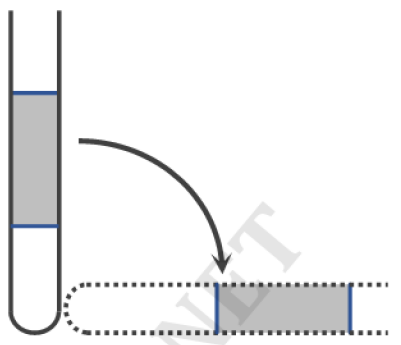
\includegraphics[scale=0.3]{img/6.png}
	\end{center}
	\choice
	{32 cm}
	{28 cm}
	{35 cm}
	{25 cm}
\end{ex}

\begin{ex}
	Một ống thủy tinh thành mỏng một đầu kín và có tiết diện đều được đặt thẳng đứng, đầu hở phía trên, cột thủy ngân dài 20 cm bịt kín cột không khí dài 49 cm. Biết áp suất khí quyển là 76 cmHg. Người ta quay ngược ống thủy tinh để đầu hở phía dưới. Chiều dài của cột không khí lúc này là
%		\begin{center}
%		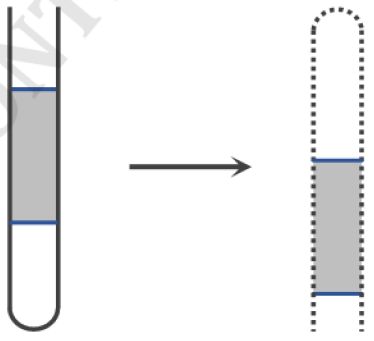
\includegraphics[scale=0.3]{img/7.png}
%	\end{center}
	\choice
	{84 cm}
	{29 cm}
	{54 cm}
	{36 cm}
\end{ex}

\begin{ex}
	Một ống thủy tinh một đầu kín, tiết diện đều, một đoạn cột không khí được bịt bởi cột thủy ngân dài 20 cm. Khi đặt ống nằm ngang thì cột không khí dài 17 cm. Khi ống nghiêng $30^\circ$ so với phương ngang với đầu hở hướng lên thì cột không khí dài 15 cm. Biết nhiệt độ của khí không đổi. Áp suất của khí quyển là
	\choice
	{72 cmHg}
	{78 cmHg}
	{81 cmHg}
	{75 cmHg}
\end{ex}

\begin{ex}
	Một ống thủy tinh một đầu kín, tiết diện đều, đặt thẳng đứng với đầu hở hướng xuống thì cột không khí có chiều dài $L$ được bịt bởi cột thủy ngân có chiều dài $h$ (cm). Biết áp suất khí quyển là $p_0$ (cmHg). Nếu nghiêng ống thủy tinh sao cho ống tạo một góc $\alpha$ với phương thẳng đứng và đầu hở phía dưới thì chiều dài của cột không khí trong ống là
	\choice
	{$\dfrac{p_0-h}{p_0-h\cos\alpha}L$}
	{$\dfrac{p_0-h}{p_0-h\sin\alpha}L$}
	{$\dfrac{p_0+h}{p_0-h\cos\alpha}L$}
	{$\dfrac{p_0+h}{p_0-h\sin\alpha}L$}
\end{ex}

\begin{ex}
	Một ống thủy tinh có chiều dài rất nhỏ so với độ sâu của bể nước, được ấn theo phương thẳng đứng (đầu hở ở dưới) từ trên mặt nước xuống đáy bể nước. Khi nhấc ống lên khỏi mặt nước thì thấy $\frac{2}{3}$ chiều dài thành trong đã bị ngâm nước. Lấy $p_a = 10^5$ Pa, $g=10 \text{ m/s}^2$, $\rho = 1000 \text{ kg/m}^3$. Coi nhiệt độ khí trong ống không đổi. Độ sâu của nước ước tính là
	\choice
	{20 m}
	{40 m}
	{60 m}
	{30 m}
\end{ex}

\begin{ex}
	Một ống thủy tinh một đầu kín tiết diện đều được cắm thẳng đứng vào một chậu thủy ngân sâu và rộng. Cột không khí trong ống lúc đầu dài 10 cm. Bề mặt thủy ngân trong ống cao hơn bề mặt thủy ngân bên ngoài ống một đoạn 70 cm. Áp suất khí quyển là 76 cmHg. Ấn từ từ ống xuống dưới theo phương thẳng đứng sao cho bề mặt thủy ngân trong ống cao hơn bề mặt thủy ngân ngoài ống một đoạn 64 cm. Lúc này, chiều dài cột không khí trong ống là
		\begin{center}
		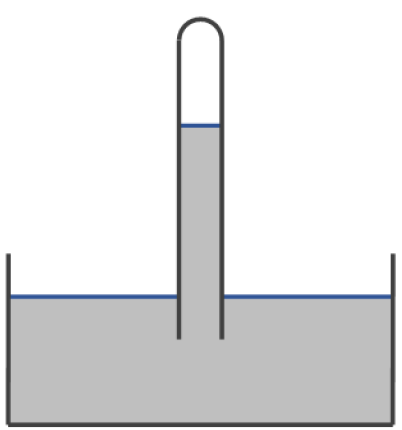
\includegraphics[scale=0.3]{img/8.png}
	\end{center}
	\choice
	{15 cm}
	{8 cm}
	{11 cm}
	{5 cm}
\end{ex}

\begin{ex}
	Một ống thủy tinh tiết diện đều, dài 1 m, có một đầu kín và một đầu hở. Giữ ống thẳng đứng (đầu hở phía dưới) rồi cắm từ từ xuống một chậu thủy ngân đến khi ống chìm trong thủy ngân 25 cm thì dừng lại. Biết áp suất khí quyển là 75 cmHg và nhiệt độ khí trong ống không đổi. Cột thủy ngân đi vào ống có chiều cao là
	\choice
	{11,6 cm}
	{12,5 cm}
	{13,4 cm}
	{14,8 cm}
\end{ex}

\begin{ex}
	Một ống thủy tinh thẳng tiết diện đều hở cả hai đầu, được cắm thẳng đứng vào một bình thủy ngân sao cho một đầu cao hơn bề mặt thủy ngân 8 cm. Áp suất khí quyển là 76 cmHg. Dùng ngón tay bịt kín đầu trên của ống rồi nâng ống thẳng đứng đi lên 46 cm. Khi đó, chiều dài cột không khí trong ống là bao nhiêu? (coi nhiệt độ cột khí trong ống không đổi).
	\choice
	{16 cm}
	{8 cm}
	{12 cm}
	{6 cm}
\end{ex}

\textbf{Phần II. Câu hỏi đúng sai.}
\setcounter{ex}{0}
\begin{ex}
	Như hình vẽ, đường cong (1) và (2) là các đường đẳng nhiệt biểu diễn liên hệ giữa áp suất $p$ và thể tích $V$ của một lượng khí xác định ở nhiệt độ $T_1$ và $T_2$ tương ứng.
		\begin{center}
		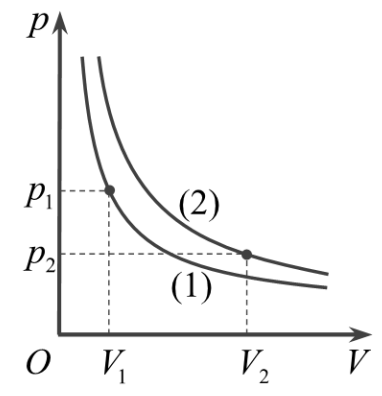
\includegraphics[scale=0.4]{img/9.png}
	\end{center}
	\choiceTF
	{$p_1 < p_2$}
	{$V_1 < V_2$}
	{$T_1 < T_2$}
	{$p_1V_1 < p_2V_2$}
 
\end{ex}

\begin{ex}
	Như hình H1, một ống hình chữ U nhỏ, tiết diện đều có chiều dài mỗi nhánh là 50 cm, chiều dài phần nằm ngang là 85 cm, nhánh trái để hở và nhánh phải kín. Chiều cao của cột thủy ngân mỗi nhánh đều là 10 cm. Biết áp suất khí quyển là 75 cmHg. Xoay ống một góc $90^\circ$ trong mặt phẳng thẳng đứng sao cho đầu hở ở trên, đầu kín dưới, hai nhánh đều nằm ngang như hình H2. Coi nhiệt độ trong cột khí kín không đổi.
		\begin{center}
		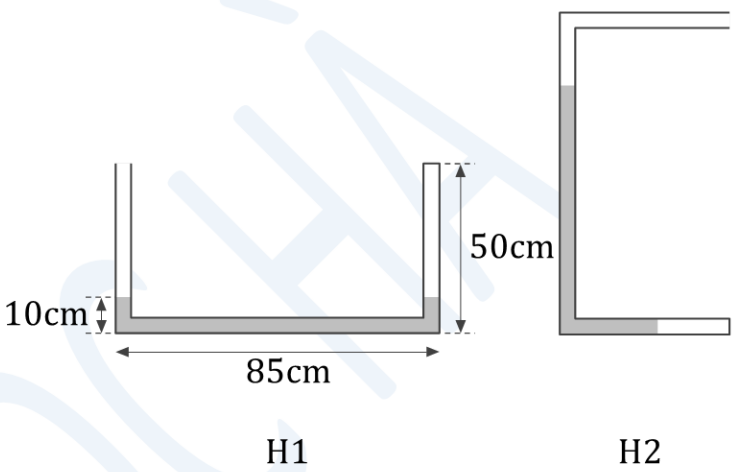
\includegraphics[scale=0.4]{img/10.png}
	\end{center}
	\choiceTF
	{Ở hình H1, cột khí kín dài 40 cm}
	{Ở hình H1, áp suất trong cột khí kín là 85 cmHg}
	{Ở hình H2, cột khí kín dài 25 cm}
	{Ở hình H2, áp suất trong cột khí kín là 150 cmHg}
\end{ex}

\textbf{Phần III. Câu hỏi trả lời ngắn.}
\setcounter{ex}{0}
\begin{ex}
	Như hình vẽ, một ống thủy tinh hình chữ U tiết diện đều có một đầu kín và một đầu hở. Bề mặt thủy ngân ở hai nhánh ngang nhau và chiều dài cột khí trong nhánh kín là $L_0 = 30$ cm. Áp suất khí quyển là 75 cmHg. Nếu đổ thủy ngân vào đầu hở sao cho chiều dài cột khí ở nhánh kín là 25 cm. Khi đó, chiều dài cột thủy ngân được đổ vào ống là bao nhiêu?
		\begin{center}
		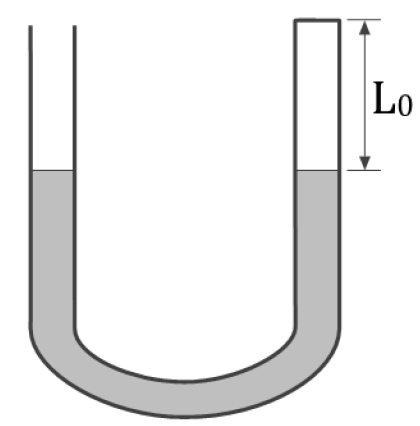
\includegraphics[scale=0.3]{img/11.png}
	\end{center}
\end{ex}

\begin{ex}
	Một ống thủy tinh thẳng tiết diện đều hở cả hai đầu, được cắm thẳng đứng vào một bình thủy ngân sao cho một đầu cao hơn bề mặt thủy ngân 27 cm. Dùng ngón tay bịt kín đầu trên của ống rồi hạ ống thẳng đứng đi xuống 8 cm. Coi nhiệt độ khí trong ống không đổi. Áp suất khí quyển là 75 cmHg. Độ cao chênh lệch giữa bề mặt thủy ngân bên trong và bên ngoài ống là bao nhiêu?
\end{ex}

\end{document}